\chapter{Dataset}\label{chapter:Dataset}

\section{Construction}
The main goal is to gather a diverse and high-quality dataset which represents static
real-world HTML/CSS webpages. This includes different layouts, components and contents. 
In the past, there have been different attempts to collect a dataset fullfilling
exactly those requirements.\newline
Two promising examples in this field are \textit{Design2Code} and \textit{Webcode2m}. 
Both have used existing, large datasets and applied different processing steps to 
filter bad examples and remove noise or redundancy from the code. Based on their
dataset curation, both serve as a good base for this thesis.\newline
Therefore, we decided to use both datasets and manually select 53 high-quality data 
entries. Those 53 data entries consist of 28 entries from Design2Code and 25 entries
from Webcode2m. In order to compare them on a fair basis, we only collect webpages 
that have english as their primary language.

\subsection{Content Distribution}
By using data entries of various domains and different layouts, we make sure to get 
a fair representation of the distribution of webpages in the real world. Based on 
our manual selection, we present the domain distribution in a pie chart in Figure 1.

\begin{figure*}[p]
  \centering
  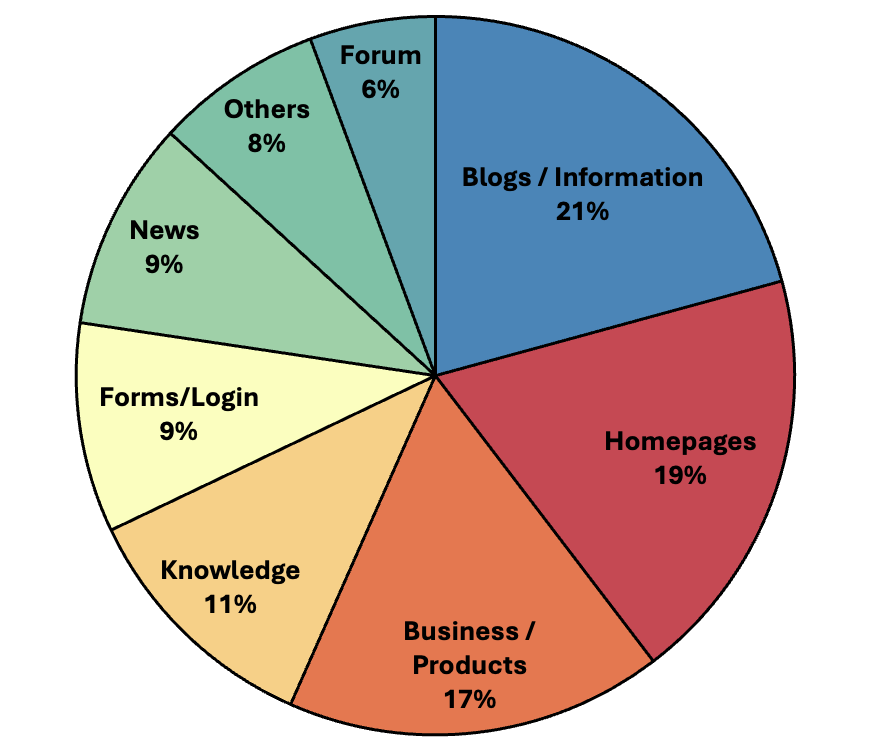
\includegraphics[width=\textwidth]{figures/dataset_distribution.png}
  \caption{Distribution of Topics in Dataset}
  \label{fig:dataset_distribution}
\end{figure*}

\section{Dataset Mutation}
Due to the fact that Design2Code and Webcode2m use different strategies to purify
their data, it is necessary to align both datasets in order to get a fair comparison.
This includes removing all external dependencies such as multimedia files (e.g. images
, audio, videos, {\ldots}) from the datasets. Furhtermore, this means adding 
placeholders like src=\"placeholder.jpg\" for images or href=\"\#\" for <a> Tags.
Lastly, we remove all of the non-visible content (advertisement-related, hidden) 
of the webpages, because it is not necessary in an Image-to-Code environment and 
could only add negatively to the accessibility score.


\section{Data Leakage}
In a last step we try to rule out the risk of data leakage. Both datasets have been
uploaded to Huggingface a few months before the official knowledge-cutoff of some of the LLMs, which
we use, and theoretically, they were publicly available at that time. 
While Design2Code has uploaded its data 3 months before the knowledge-cutoff, in the 
case of Webcode2m, it was only 2 months. To tackle this issue, we create a 
new, leakage-proof dataset of 20 entries which we input to the LLMs and compare their 
performance. If the performance in terms of our Benchmarks is comparable to our the one 
of our existing dataset, we assume that no data leakage has occurred.\newline
This test dataset has 20 data entries and has been collected the following way:

\begin{itemize}
  \item \textbf{Mutation of old Data:} We use 10 randomly-selected data entries of our existing 
  dataset. 
  \item \textbf{Collection of new Data:} The other 10 data entries have been collected from 
  two Github repositories which contain frontend webpages. Those webpages have been crawled 
  and added to the dataset.
\end{itemize}

\subsection{Mutation of old Data}
The mutation of the data entries tries to change the existing ones without losing the 
reference to the real-world. The goal is to change the data entries in such a way, that
the LLMs cannot memorize the data entries, without adding artificial noise or new 
accessibility violations. Therefore, we apply the following mutations to the data entries:

\begin{itemize}
  \item \textbf{Text:} The entire text has been rewritten by a LLM. While the meaning
    and the length (max ±20 \%) remains roughly the same, the wording changes
    completely, in order to avoid memorization based on text snippets.
  \item \textbf{Text Font:} To change the visual appearance of the data entries, we 
    define a set of 5 commonly used fonts in webpages. Based on a random sample, we 
    change the text font for each data entry.
  \item \textbf{Colors:} The \textit{HUE} color code of each element is slightly
    changed based on a random shift (±20 degrees). Apart from that, the saturation
    and lightness of the color is changed by a maximum of ±20 \%.
\end{itemize}

Since those changes remain quite superficial and might not be enough to rule out 
data leakage, we further alter those data entries. We randomly change the structure 
of the data entries manually. Components, such as tables, images and text are 
interchanged within one html/css file in order to alter the webpage's layout.
Apart from that, we implement cross-web exchanges, similar to former research (paper).
We randomly select an order and exchange header and footer within different files. 
This ensures a completely new layout, while making sure that the new data entries 
remain realistic and similar to their real-world parents.

\subsection{Collection of new Data}
In a second step we collect webpages of two Github repositories which have been 
created in 2025. The first repository (source) is an educational project 
with many different webpage styles and layouts. The second repository (source)
offers a wide range of e-commerce related webpages. \newline
We crawl their html/css, pay attention on diverse content and randomly select
10 examples of this pool.


\subsection{Results}
The final results can be seen in the appendix. However, they show no difference 
in terms of the benchmarks between the existing dataset and this new leakage-free 
dataset. Since we do not have any evidence for data leakage, we assume that the 
LLMs have not seen the existing data and therefore continue with the tests.


